\section{Method}\label{sec:method}



In this section, we first provide an overview of MemSkill (Section~\ref{sec:method_overview}), then detail the \emph{skill bank} (Section~\ref{sec:skill_bank}) and the three core components (\emph{controller} (Section~\ref{sec:controller}), \emph{executor} (Section~\ref{sec:executor}), and \emph{designer} (Section~\ref{sec:designer})), and finally summarize the closed-loop optimization procedure that alternates between learning to use the current skills and evolving the skill bank from hard cases (Section~\ref{sec:closed_loop}).


\begin{figure*}[t]
	\centering
	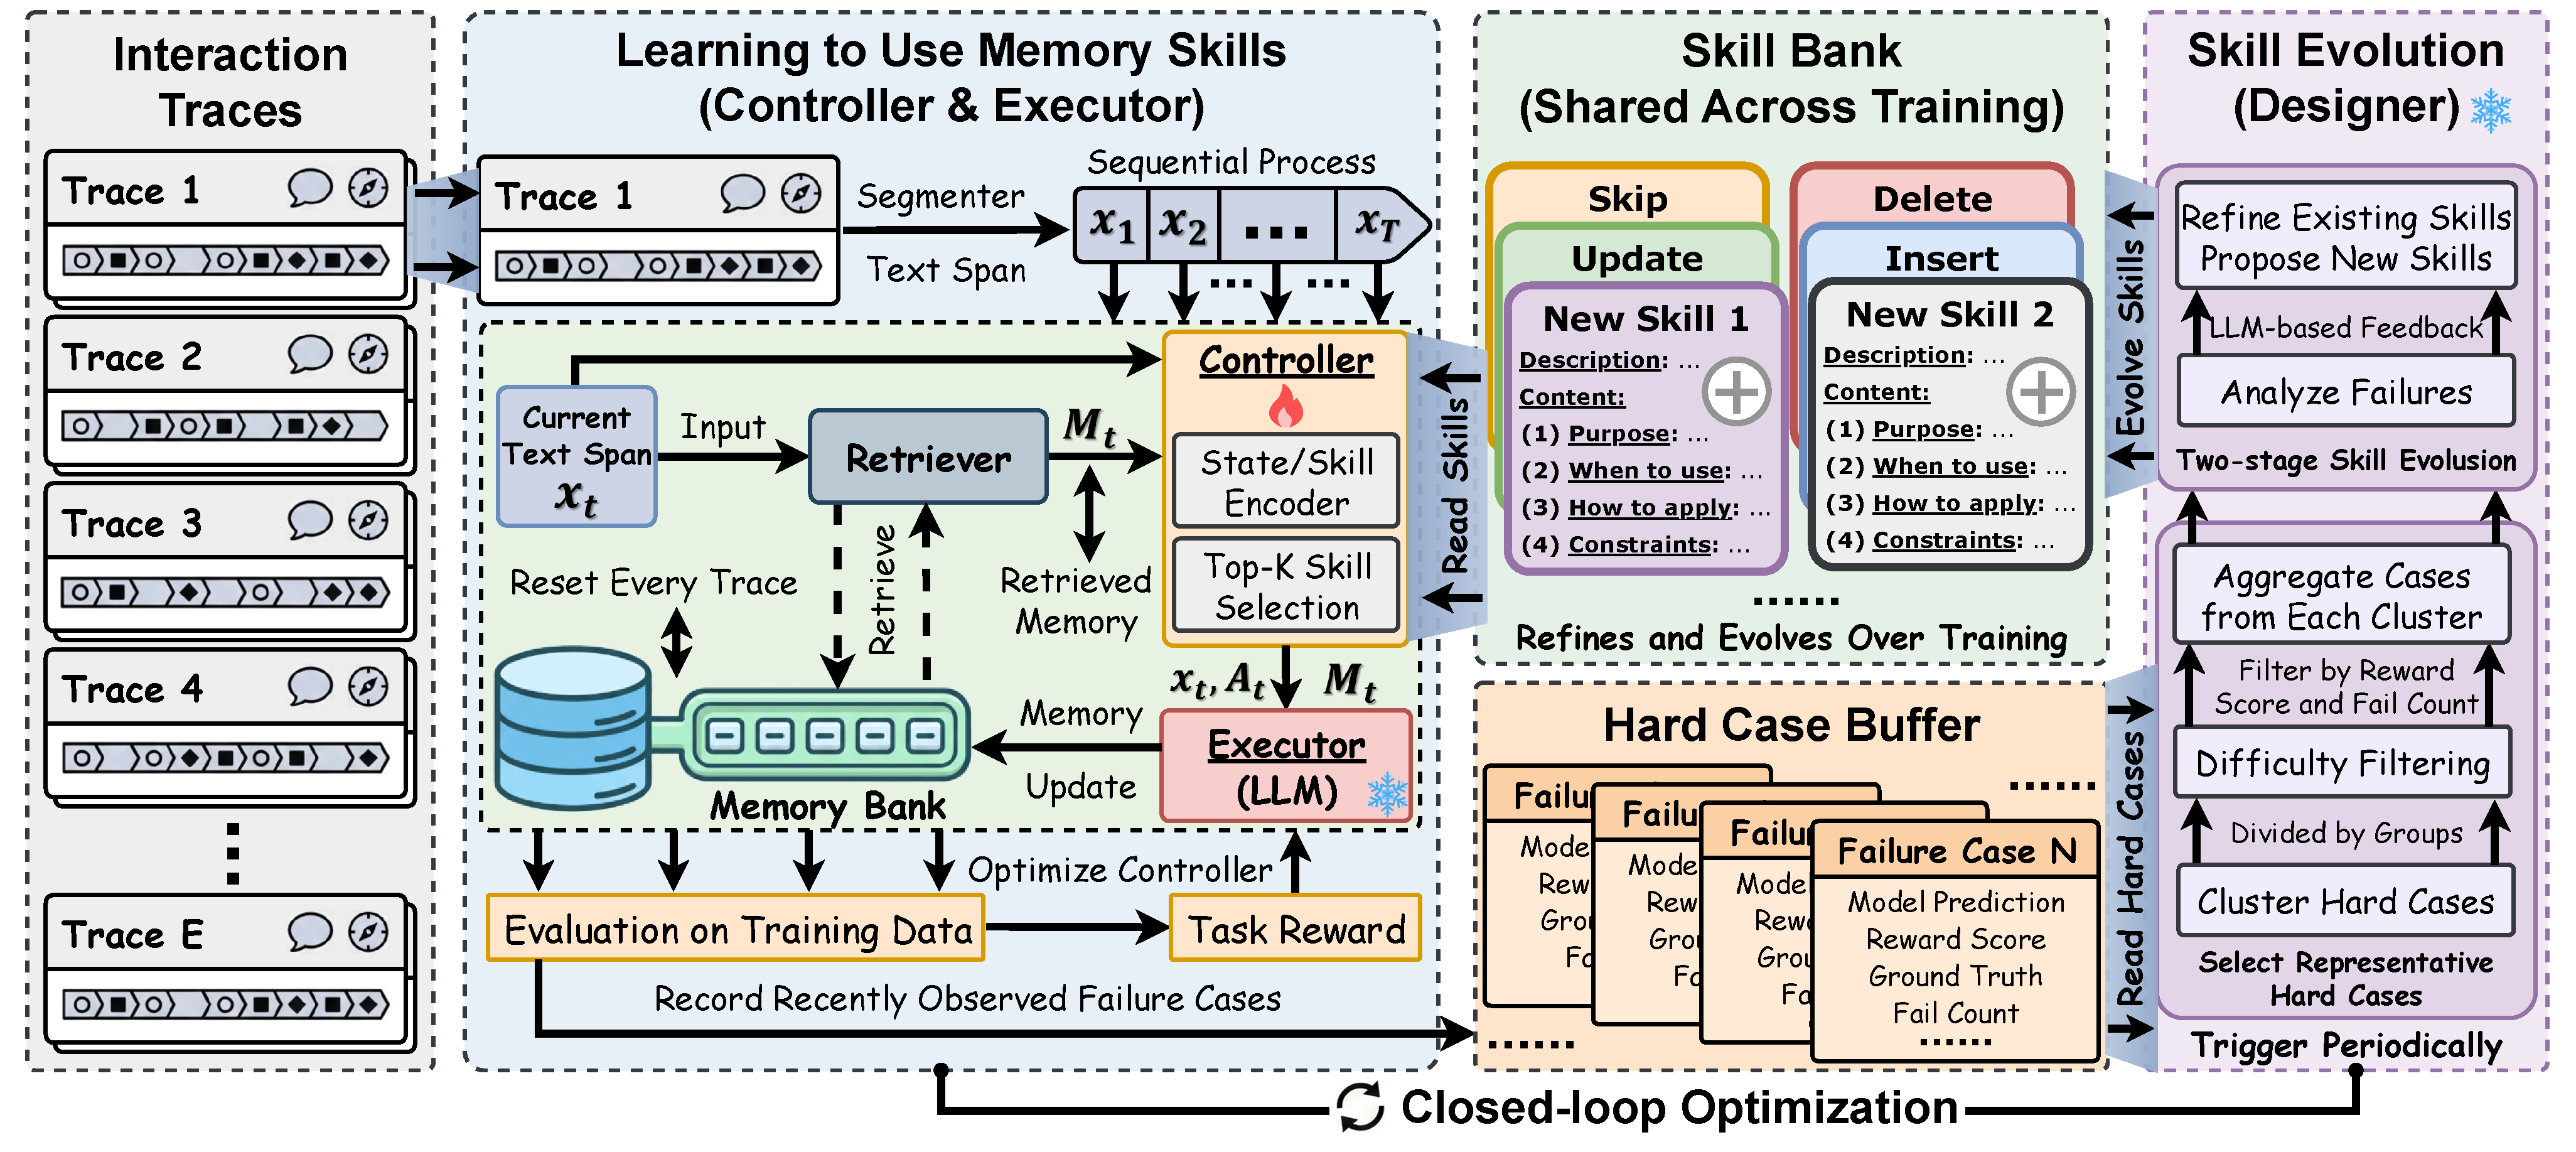
\includegraphics[width=1.0\linewidth]{figs/skill_method.pdf}
        \caption{\textbf{MemSkill architecture overview.} Given an interaction trace, MemSkill processes it span by span: the controller selects a Top-$K$ subset of skills from a shared \emph{skill bank} conditioned on the current text span and retrieved memories, and an LLM executor applies the selected skills in one pass to update the trace-specific \emph{memory bank}. The constructed memory is then evaluated on memory-dependent training queries to provide task reward for optimizing the controller, while query-centric failures are logged into a sliding hard-case buffer. Periodically, the designer mines representative hard cases to refine existing skills and propose new ones, yielding alternating phases of skill usage and skill evolution. More skill case study can be found in Section~\ref{sec:case_study} and Appendix~\ref{appendix:case_study}.}
	\label{model_figure}
\end{figure*}






\subsection{Overview}\label{sec:method_overview}



As shown in Figure~\ref{model_figure}, we propose \textbf{MemSkill}, which optimizes agent memory through two intertwined processes. First, it \textbf{learns to use a given skill bank}: a controller selects context-relevant skills, and an executor applies them to produce memory updates. Second, it \textbf{improves the skill bank itself}: a designer periodically revises existing skills and adds new ones based on challenging training cases.




To disentangle trace-specific memories from reusable memory management knowledge, MemSkill maintains two stores. 
The \emph{memory bank} is trace-specific and stores memories for each training trace (e.g., a long dialogue). 
In contrast, the \emph{skill bank} is shared across traces and contains reusable memory skills.
During training, the controller and executor build each trace's memory bank, while the designer updates the shared skill bank between phases. This alternating procedure gradually improves both the skill selection policy and the skill bank for memory construction.




\subsection{Skill Bank}\label{sec:skill_bank}



As shown in Figure~\ref{model_figure}, a \emph{memory skill} specifies a reusable memory operation as structured guidance, including when it is applicable and how it should be applied to the current context. Concretely, each skill $s \in \mathcal{S}$ contains (i) a short \emph{description} for skill representation and selection, and (ii) a detailed \emph{content} specification that instructs the executor on memory extraction or revision.




We start from a minimal set of general-purpose primitives to ensure a stable and functional initialization. Specifically, we initialize the skill bank with four basic skills corresponding to canonical memory operations: \textsc{Insert}, \textsc{Update}, \textsc{Delete}, and \textsc{Skip}. Starting from this minimal set, the designer progressively refines existing skills and expands the bank by proposing new skills that address uncovered failure modes. (Appendix~\ref{appendix:case_study} details skill description)




\subsection{Learning to Use Memory Skills}\label{sec:learn_to_use_skills}

In this part, we describe how MemSkill learns to use memory skills, covering (i) the skill-selection policy and (ii) skill-conditioned memory construction.



\subsubsection{Controller: Skill Selection Policy}\label{sec:controller}




To enable effective skill selection as the \emph{skill bank} evolves, we introduce a controller that selects a small set of relevant memory skills for the current context. 
At each memory construction step, \textbf{we update memory at the span level}: we split each interaction trace (e.g., a dialogue) into fixed-length contiguous spans by token count and process them sequentially. For each span, the controller conditions its selection on (i) the current text span and (ii) the retrieved existing memories from the current trace's memory bank (empty for initial span), rather than operating turn by turn.




To remain compatible with a variable-size skill bank as it continuously evolves, the controller scores each skill by measuring the semantic distance between the current state and skill representations, supporting a changing skill set while staying sensitive to what is already stored in memory.




\textbf{State and skill representations.}
Formally, let $x_t$ denote the current text span at step $t$, and let $M_t=\{m_{t,1},\dots,m_{t,R}\}$ be the retrieved memories from the current trace's memory bank. We first encode $x_t$ and $M_t$ with a fixed embedding model $e(\cdot)$, aggregate the retrieved memory embeddings by element-wise averaging, and concatenate it with the span embedding:
\begin{equation}
h_t = f_{\theta}^{\mathrm{ctx}}\!\left([e(x_t);\bar{m}_t]\right), \qquad
u_i = f_{\theta}^{\mathrm{skill}}\!\left(e(\mathrm{desc}(s_i))\right),
\end{equation}
where $\bar{m}_t=\frac{1}{R}\sum_{r=1}^{R}e(m_{t,r})$ denotes the aggregated memory embedding, and is omitted when $M_t$ is empty. Here, $u_i$ is the representation of skill $s_i \in \mathcal{S}_t$, computed from its description as a compact and stable semantic signal rather than the full skill content. The embedding model $e(\cdot)$ is shared and fixed, while $f_{\theta}^{\mathrm{ctx}}$ and $f_{\theta}^{\mathrm{skill}}$ are trainable neural networks in the controller for learnable skill selection.





\textbf{Compatibility with an evolving skill bank.}
Instead of producing a fixed-dimensional action head tied to a fixed number of skills, the controller concatenates the state representation with each candidate skill representation and applies a shared scorer to all such state-skill pairs in parallel:
\begin{equation}
z_{t,i} = f_{\theta}^{\mathrm{score}}\!\left([h_t;u_i]\right), \qquad
p_\theta(i \mid h_t) = \mathrm{softmax}(z_t)_i,
\end{equation}
where $f_{\theta}^{\mathrm{score}}$ is a trainable neural network, and $z_t \in \mathbb{R}^{|\mathcal{S}_t|}$ adapts as the skill bank evolves.




\textbf{Top-$K$ skill selection.}
Given the categorical distribution $p_\theta(i\mid h_t)$ over the current skill bank $\mathcal{S}_t$, the controller selects an ordered Top-$K$ set of skills
$A_t=(a_{t,1},\dots,a_{t,K})$ (e.g., via Gumbel-Top-$K$~\citep{kool2019stochastic}), and only passes the selected skills to the executor, keeping the skill context concise and relevant.





\subsubsection{Executor: Skill-Conditioned Memory Extraction}\label{sec:executor}






Given the selected skills $A_t$, the fixed executor constructs memory updates by conditioning an LLM on (i) the current text span $x_t$, (ii) the retrieved memory items $M_t$, and (iii) the selected skills $A_t$. This mirrors skill-conditioned inference in agent systems, where a small set of relevant skills is provided to guide behavior for the current context.
The executor produces structured memory updates, which are parsed and applied to the trace's memory bank. 
By composing several skills for the same text span and extracting memory in one LLM call, MemSkill reduces repeated per-turn processing and scales better to long interaction histories.
Appendix~\ref{appendix:prompts} details the executor prompt.




\subsubsection{Controller Optimization}\label{sec:controller_optimization}


We train the controller with reinforcement learning, using downstream task performance as feedback for its skill selections. For each training trace, the controller makes a sequence of Top-$K$ selections while the executor incrementally builds the trace-specific memory bank. After construction, we evaluate the resulting memory bank on the trace's memory-dependent training queries and use the resulting task performance as the reward (e.g., F1 or success rate).





A key technical detail is that the controller's action is an ordered Top-$K$ \emph{list} selected without replacement, rather than a single discrete action. We therefore compute the joint log-probability $\log \pi_\theta(A_t\mid h_t)$ under this selection process and use it in standard policy-gradient objectives~\citep{schulman2017proximal} via importance weighting and clipping. Concretely, for $A_t=(a_{t,1},\dots,a_{t,K})$, the joint probability is
\begin{equation}
\pi_\theta(A_t \mid h_t)
= \prod_{j=1}^{K}
\frac{p_\theta(a_{t,j}\mid h_t)}
{1-\sum_{\ell<j} p_\theta(a_{t,\ell}\mid h_t)} ,
\label{eq:topk_joint_prob_main}
\end{equation}
which reduces to the single-action case when $K=1$. Appendix~\ref{appendix:rl_objective} gives implementation details.




\subsection{Skill Evolution through Designer Feedback}\label{sec:designer}


Beyond learning to select from a fixed set of skills, MemSkill evolves the skill bank using an LLM-based designer (fixed) that operates periodically during training.

\textbf{Hard-case buffer.} During controller training, we maintain a sliding-window buffer of challenging cases observed recently. Each case is query-centric, recording the query along with its ground-truth and metadata (e.g., retrieved memories and model prediction), as well as summary statistics such as task performance and the number of failures observed so far.
The buffer uses two expiration rules: cases are removed if they become too old (exceeding a maximum training step gap) or if the buffer reaches its capacity limit, which tracks recent failure patterns without growing unbounded.

\textbf{Selecting representative hard cases.} To focus designer updates on impactful failures, we cluster cases (e.g., KMeans) into groups that naturally reflect different query or error types. Within each cluster, we prioritize representative cases using a difficulty score that increases when task performance is low and when the same case fails repeatedly. This produces a compact set of high-value cases for skill evolution while preserving diversity across error types. 



\textbf{Two-stage skill evolution.} The designer updates the skill bank in two stages. First, it employs an LLM to analyze the selected hard cases and identify what memory behaviors are missing or mis-specified. Second, it uses the resulting analysis to propose concrete edits to existing skills and to introduce new skills. We keep the designer description concise and provide prompts in Appendix~\ref{appendix:prompts}.





Notably, we maintain snapshots of the best-performing skill bank and roll back if an update degrades performance, with early stopping when repeated designer updates fail to improve the training signal. After each evolution step, we also briefly increase exploration by biasing selection toward newly introduced skills, encouraging the controller to try them and facilitating efficient learning of their utility.
Due to page limit, more details about the designer can be found in Appendix~\ref{appendix:detail_component}.



\subsection{Closed-Loop Optimization}\label{sec:closed_loop}


MemSkill alternates between (i) learning to select and apply skills to build memory banks and (ii) evolving the skill bank from hard cases mined during training. Each cycle begins with controller training on the current skill bank, where the executor constructs memories and accumulates challenging cases. The designer then updates the skill bank using representative hard cases, optionally rolling back to a prior snapshot if performance regresses. The next cycle resumes controller training on the updated skill bank, with additional exploration to encourage early use of new skills. Over cycles, this closed loop gradually improves how skills are selected, applied, and refined for memory construction.



